\section{Realisatie}

\subsection{Spanningsreferentie}
Zoals besproken in \cref{sec:referenceVoltage} kunnen de weerstandswaardes van de spanningsreferentie erg hoog gekozen worden. Met een $R_1$ van \qty{5.6}{\mega\ohm} gebruikt de spanningsdeler \qty{1.65}{\micro\watt}.

Volgens \cref{eq:dividerNoise} heeft de condensatorwaarde wel effect op de ruis. Met een condensator van \qty{1}{\micro\farad} produceert de spanningsreferentie \qty{64.4}{\nano\volt} aan ruis. Dit zorgt voor een signaal-ruis verhouding van \qty{138}{\decibel}, wat meer dan genoeg is.

Deze gekozen waardes en de resulterende eigenschappen zijn te vinden in \cref{tab:divider}.

\begin{table}[ht]
\centering
\begin{tabular}{l|l|l}
    Symbool & Waarde & Eenheid \\
    \hline
    $R_1$       & 5.6  & $\si{\mega\ohm}$   \\
    $R_2$       & 1.0  & $\si{\mega\ohm}$   \\
    $C$         & 1.0  & $\si{\micro\farad}$\\
    $P$         & 1.65 & $\si{\micro\watt}$ \\
    $u_{n,out}$ & 64.4 & $\si{\nano\volt}$  \\
    SNR         & 138  & $\si{\decibel}$
\end{tabular}
\caption{De gekozen waardes van de spanningsdeler, met het resulterende vermogensverbruik en de ruiseigenschappen.}
\label{tab:divider}
\end{table}

\subsection{Microcontroller}
Het is erg belangrijk om een energiezuinige microcontroller te kiezen. Het digitale gedeelte van het energieverbruik kan opgedeeld worden in 3 onderdelen: de ADC, de digitale signaalverwerking (\cref{fig:digitaleBewerkingsFunctie}) en het draadloos versturen van data. Het is mogelijk om elk van deze onderdelen met een apart component te doen. Er zijn echter ook componenten beschikbaar die elk van deze functionaliteiten zelf al bevatten.

Een voorbeeld hiervan is de nRF52810. Deze microcontroller heeft 14 bit (met oversampling) ADC kanalen en een ingebouwde 2.4GHz Bluetooth transceiver. 

% rf implementatie, is industrie standaard, rtos support??, 

\subsection{ADC}
De ADC die in de \mcu  zit ingebouwd voldoet aan de specificaties in \cref{tab:specADC,tab:systemSpecADC}\cite{nrf52810}. Het is dus niet nodig om een externe ADC te gebruiken. 


\subsection{Filter}
Het laagdoorlaatfilter dat voor de ADC zit, heeft een weerstand en een condensator die van een waarde voorzien moeten worden.
Met de ruis van het voorgaande systeem kan de minimale condensatorwaarde berekend worden door middel van \cref{eq:filterCapMin}. Deze komt uit op ongeveer \qty{60}{\pico\farad}. Hiermee moet de weerstandswaarde echter \qty{270}{\mega\ohm} zijn, wat niet praktisch is. Met een condensator van \qty{10}{\nano\farad} kunnen de waardes in \autoref{tab:filterValues} berekend worden. Deze waardes vallen binnen de specificaties.

\begin{table}[ht]
    \centering
    \begin{tabular}{l|l|l}
        Symbool & Waarde & Eenheid \\
        \hline
        $C$         & 82    & $\si{\nano\farad}$\\
        $R$         & 180   & $\si{\kilo\ohm}$  \\
        $f_c$       & 10.8  & $\si{\hertz}$     \\
        $P$         & 408   & $\si{\nano\watt}$ \\
        $u_{n,out}$ & 225   & $\si{\nano\volt}$ \\
        NF          & 0.23  & $\si{\decibel}$   \\
    \end{tabular}
    \caption{De gekozen waardes van het filter, en de resulterende vermogens- en ruiseigenschappen.}
    \label{tab:filterValues}
\end{table}


\subsection{Nullor implementatie}
Voor de nullor die gebruikt wordt om de ISFET uit te lezen in \cref{sec:ISFETLees} moet een implementatie gekozen worden. De uitleesschakeling mag volgens de specificaties maximaal \qty{200}{\micro\watt}  gebruiken. De constante stroom die door de weerstand en ISFET in \cref{fig:measureResistor} heen loopt, zorgt voor een constant vermogensverbruik van \qty{165}{\micro\watt}. Hierdoor mag de nullor implementatie maximaal \qty{35}{\micro\watt} gebruiken. Het maximale dynamische vermogen dat deze nullor implementatie aan de uitgang zal moeten kunnen leveren, is gelijk aan het maximale vermogen dat het filter kan dissiperen. Er blijft dan afgerond nog \qty{34}{\micro\watt} aan statisch vermogen over. Dit resulteert in een maximale quiescent stroom van \qty{10.3}{\micro\ampere}.

De uitleesschakeling moet een minimale SNR hebben van 40 dB. De maximale ruisspanning en stroom die de nullor mag genereren aan de ingang zijn te berekenen met \cref{eq:nullorImplementNoise}. Deze vergelijking is afgeleid uit \Cref{eq:measureNoiseFull}.
\begin{equation} \label{eq:nullorImplementNoise} 
    S_{u_{{n,n}}} + S_{i_{{n,in}}}\left(Z_{fet} // R\right)^2 = \frac{S_{u_{{n,out}}}}{H^2(\ph)} - S_{u_{{n,ref}}}
\end{equation}

De LTC2064 opamp heeft (buiten shutdown) een quiescent stroom van \qty{2.5}{\micro\ampere}, wat op 3.3 V resulteert in een vermogen van \qty{8.25}{\micro\watt}. Daarbij heeft deze een spectrale ruisdichtheid van \qty{12}{\femto\ampere\hertz^{-0.5}} en $\qty{220}{\nano\volt\hertz^{-0.5}}$\cite{LTC2064}. Dit zit volgens \cref{eq:nullorImplementNoise} ver onder het maximum. Daarbij is zowel de ingangsafwijking als de 1/f ruis van deze opamp erg laag. Hierdoor is deze opamp gekozen voor het ontwerp.

\subsection{Rf}


\subsection{Voeding}
% software 
% hardware

\subsection{Printplaten}
De schakelingen voor de voeding en voor het uitlezen van de ISFET zijn opgedeeld in twee verschillende printplaten. Dit is gedaan zodat beide schakelingen apart van elkaar getest kunnen worden. De uitlees printplaat (\cref{fig:sensorPCB}) bevat de ISFET uitleesschakeling, samen met de \mcu, die de gemeten pH waarde verzendt. De voeding printplaat (\cref{fig:powerPCB}) regelt de energy harvesting, samen met het veilig opladen en het ontladen van de batterij. De twee printplaten zijn met elkaar verbonden door middel van pin headers. Beide schakelingen zijn te zien \cref{fig:PCBs}.

Beide PCB's hebben op elk belangrijk signaal een testpunt zitten. Op deze manier kan er eenvoudig gemeten worden.


\begin{figure}[ht]
    \centering
    \begin{subfigure}[b]{0.48\textwidth}
        \centering
        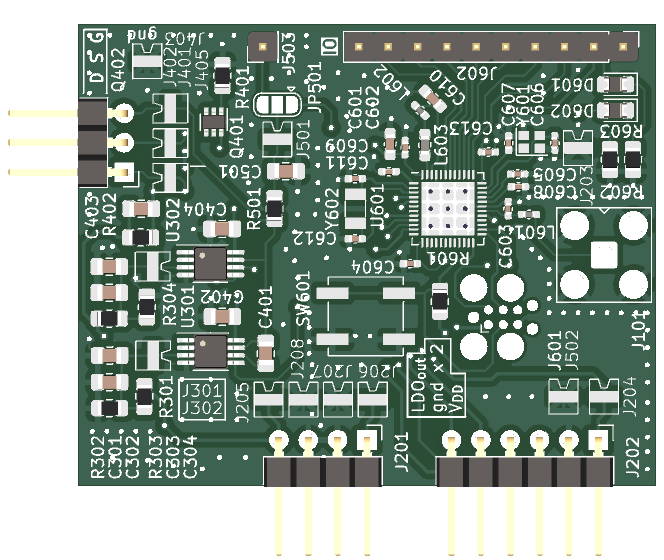
\includegraphics[width=\textwidth]{sensorBord}
        \caption{De ISFET uitlezer PCB.} 
        \label{fig:sensorPCB}
    \end{subfigure}
    \hfill
    \begin{subfigure}[b]{0.60\textwidth}
        \centering
        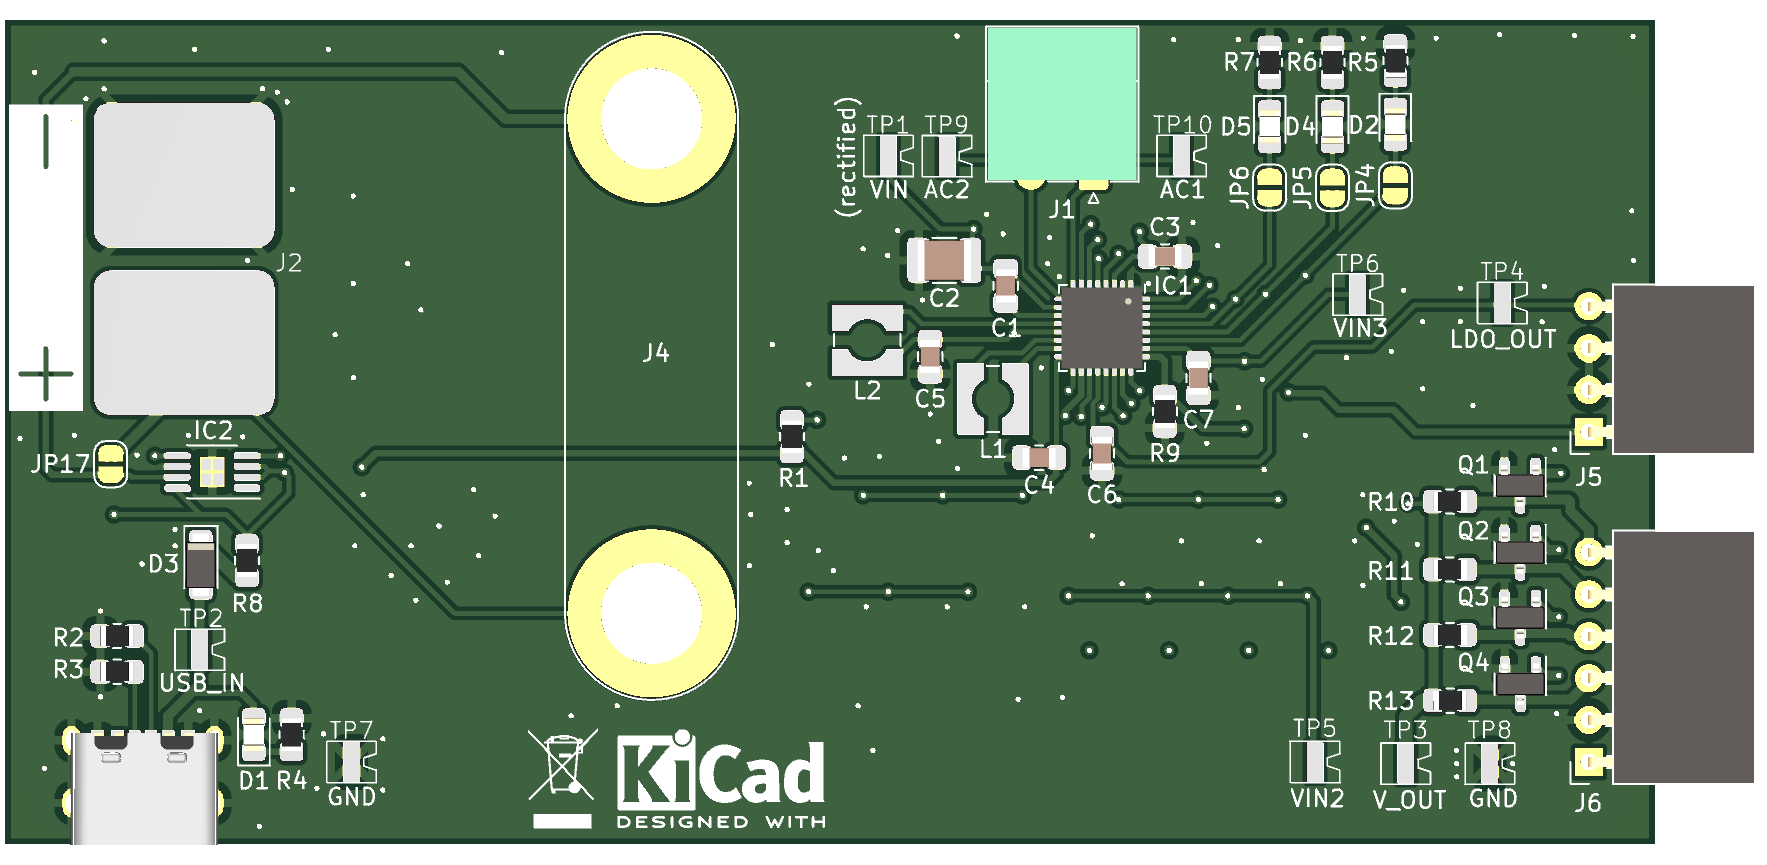
\includegraphics[width=\textwidth]{powerandharvest}
        \caption{De voeding en harvesting PCB.} 
        \label{fig:powerPCB}
    \end{subfigure}
    \caption{De gemaakte PCB's.}
    \label{fig:PCBs}
\end{figure}